%%% Documento tipo para trabajos en LaTeX.
%%% Copyleft: Jesús Balsa, Juan F. García.


% Tipo de documento:
\documentclass[12pt,a4paper,onecolumn,oneside]{report}
\newcommand{\mychapter}[2]{
	\setcounter{chapter}{#1}
	\setcounter{section}{0}
	\chapter*{#2}
	\addcontentsline{toc}{chapter}{#2}
}



% Opcional: Tamaño personalizado para los márgenes:
\usepackage[a4paper, top=3cm, bottom=3cm, left=3cm, right=3cm]{geometry}

\usepackage[utf8]{inputenc} % Codificación UTF-8.
\usepackage[T1]{fontenc}    % Para usar caracteres con tilde.
\usepackage[spanish,es-tabla]{babel} % Escritura en castellano.
\usepackage{eurosym}  % Para el símbolo del EURO (€).
\usepackage{graphicx} % Paquete de imágenes, para introducir figuras.
\DeclareGraphicsExtensions{.pdf,.png,.jpg}
\usepackage[usenames,dvipsnames]{color} % Texto en colores.
\usepackage{xcolor}   % Extra colors.
\usepackage{url}      % Para escritura de URLs.
\usepackage[breaklinks]{hyperref} % Hiperreferencias.
\usepackage{amsmath,amssymb} % Para los símbolos matemáticos.
\usepackage{cite}     % Para las citas de referencias (crea el superíndice).
\usepackage{listings} % Para coloreado de código fuente.
\usepackage{verbatim} % Para textos tipo consola y otros formatos.
\usepackage{fancyvrb} % Más opciones de verbatim.
\usepackage{parskip}  % OPCIONAL: Separa los párrafos con una línea en blanco.
\setlength{\parindent}{15pt} % Sangría de párrafos estándar (15 puntos). Necesario incluirla si se usa el paquete 'parskip'.
\usepackage[export]{adjustbox}
\usepackage{caption}  % Para personalizar los pies de foto.

% Opciones del paquete caption para los pies de imágenes y tablas:
\captionsetup{figurename=Figura, tablename=Tabla, labelsep=colon, labelfont=bf, font=small, justification=centering}

% Para el control de líneas viudas y huérfanas (líneas sueltas en páginas nuevas):
\usepackage[all]{nowidow}

\usepackage[nottoc]{tocbibind}    % Incluye el apartado "Referencias" en el índice.
%\def\spanishrefname{Bibliografía} % Para que ponga "Bibliografía" en lugar de "Referencias". SÓLO se aplica a formato "article". En "report" ya pone "Bibliografía".

\usepackage{fancyhdr}


\setlength{\unitlength}{1 cm} % Unidad de trabajo de medidas.

\renewcommand*{\baselinestretch}{1.25} % Altura del INTERLINEADO.
\renewcommand{\shorthandsspanish}{}    % Para que corte las palabras según el castellano.


% Propiedades para el PDF generado (METADATOS):
\newcommand{\authorNames}{Nombre y apellidos del autor}
\newcommand{\pdftitle}{Título del trabajo}
\hypersetup{
  pdftitle={\pdftitle},% Título
  pdfauthor={\authorNames},% Autor
  pdfsubject={\pdftitle \ - \authorNames},% Asunto
% pdfkeywords={Opcional: algunas palabras clave}%
}

% Para la representación de código fuente:
% Para BASH:
\lstset{
	language=bash,
	basicstyle=\scriptsize,
	frame=single,
	numbers=left,
	numberstyle=\scriptsize,
	stepnumber=1,
	numbersep=9pt,
	backgroundcolor=\color{White},
	showspaces=false,
	showstringspaces=false,
	showtabs=false,
	tabsize=4,
	captionpos=b,
	breaklines=true,
	keywordstyle=\color{blue}\bfseries,
	%identifierstyle=\color{green}\bfseries,
	stringstyle=\color{orange}\bfseries,
	commentstyle=\color{gray}\bfseries
}
% Para C++:
%\lstset{
%	language=C++,
%	frame=single,
%	keywordstyle=\color{Green}\bfseries,
%	identifierstyle=\color{BlueViolet},
%	stringstyle=\color{Red},
%	commentstyle=\color{MidnightBlue}
%}

\usepackage{fancyhdr} % Para el tamaño y estilo de los encabezados.

\fancypagestyle{headings}{% Redefine el estilo "headings".
	\fancyhf{} % Clear all header and footer fields.
	\lhead{\small \it Máster Universitario en Investigación en Ciberseguridad} 
	\rhead{\small \it Página \thepage}      % Nº de página a la derecha. Tamaño "small".
	\renewcommand{\headrulewidth}{1pt}
}

% Ajustes para división manual de palabras:
\hyphenation{Python} % Impide que la palabra Python sea dividida al acabar una línea.



%%%%%% INICIO DEL DOCUMENTO: %%%%%%

\begin{document}

% Página de TÍTULO (portada):
\begin{titlepage}

\begin{picture}(0,0)
\put(0,0){
\includegraphics[height=3cm]{figuras/ule.jpg}}
%\put(10,0){\includegraphics[width=3cm,height=4cm]{figuras/inf.jpg}}
\end{picture}

\begin{center}
\textbf{{\Large \bf Departamento de Matemáticas}}\\[7cm]  % Salto de línea dejando 1.2cm.
{\Large \bf MÁSTER UNIVERSITARIO EN INVESTIGACIÓN EN CIBERSEGURIDAD}\\[2.5cm]
{\Large Trabajo de Fin de Máster}\\[2.5cm]
{\Large \textbf{TÍTULO DEL TRABAJO\\[0.7cm]
TITLE OF THE WORK\\[2.5cm]}}
\end{center}

\begin{flushright}
{\bf Autor: Nombre y apellidos del autor}\\[0.5cm]
{\bf Tutor: Nombre y apellidos del tutor}\\[1.4cm]
\end{flushright}

\end{titlepage}


% Página de FIRMAS:
\newpage

\thispagestyle{empty} % para que no se numere esta página.

\begin{center}
\Huge{(Mes, Año)}
\end{center}

\begin{table*}[ht]
		\centering
		\makebox[\textwidth]{
			\begin{tabular}{|l|l|}
				\cline{1-2}
				\multicolumn{2}{|c|}{}	\\
				\multicolumn{2}{|c|}{\textbf{UNIVERSIDAD DE LEÓN}}	\\
				\multicolumn{2}{|c|}{\textbf{Departamento de Matemáticas}}	\\ 
				\multicolumn{2}{|c|}{\textbf{MÁSTER UNIVERSITARIO EN INVESTIGACIÓN EN CIBERSEGURIDAD}}	\\
				\multicolumn{2}{|c|}{\textbf{Trabajo de Fin de Máster}}	\\ 
				\multicolumn{2}{|c|}{}	\\ \hline
				\multicolumn{2}{|l|}{\textbf{ALUMNO}: Nombre y apellidos del alumno}	\\ \hline
				\multicolumn{2}{|l|}{\textbf{TUTOR}: Nombre y apellidos del tutor}	\\ \hline
				\multicolumn{2}{|p{16cm}|}{\textbf{TÍTULO}: Título del Trabajo Fin de Máster} \\ \hline
				\multicolumn{2}{|p{16cm}|}{\textbf{TITLE}: Title of the work} \\ \hline
				\multicolumn{2}{|l|}{\textbf{CONVOCATORIA}: Mes, año}		\\ \hline
				\multicolumn{2}{|l|}{\textbf{RESUMEN}:} \\ 
				\multicolumn{2}{|l|}{}\\
				\multicolumn{2}{|p{16cm}|}{El resumen reflejará las ideas principales de cada una de las partes del Trabajo Fin de Máster pudiendo incluir un avance de los resultados obtenidos. Constará de un único párrafo y se recomienda una longitud no superior a 300 palabras. En cualquier caso esta Hoja de Datos no deberá superar una página de longitud.} \\ 
				\multicolumn{2}{|l|}{}\\
				\hline
				\multicolumn{2}{|l|}{\textbf{Palabras clave}: Lorem, ipsum, dolor, sit, amet..}	\\ \hline
				\textbf{Firma del alumno}:\hspace{40mm} & \textbf{VºBº Tutor:}\\ 
				 & \\
				 & \\
				 & \\
				 & \\
				\hline
			\end{tabular}
		}
	\end{table*}



\newpage
\pagestyle{plain}

\renewcommand{\thepage}{\roman{page}}
\setcounter{page}{1} % Esta página es la 1.


% Página con el ÍNDICE GENERAL
\tableofcontents

% Página con el ÍNDICE DE FIGURAS
\listoffigures

% Página con el ÍNDICE DE TABLAS
\listoftables

% Página con el GLOSARIO:
\mychapter{0}{Glosario de términos}
\label{chap:glosario}
% A partir de aquí ya se incluye el encabezado en las páginas:
\pagestyle{headings}

% Al ser un capítulo sin número, hay que indicarle qué título añadir al encabezado de la página:
\markboth{GLOSARIO}{} 



Catálogo de términos específicos del contexto del trabajo.


\begin{description}
	
	\item[ciberseguridad]: Protección de los sistemas informáticos y de sus redes de comunicaciones, con el objetivo de mantener segura la información que procesan.
	
	\item[DES]: Data Encryption Standard. Es un algoritmo criptográfico, de tipo cifrado por bloque.
	
	
\end{description} 

%%%% Inicio de los CAPÍTULOS %%%%
\newpage
\renewcommand{\thepage}{\arabic{page}}
\setcounter{page}{1} % Esta página es la 1.

\mychapter{0}{Introducción}
\label{Introducción}

NFC significa Near Field Communication, comunicación de campo cercano. Es una plataforma abierta de comunicación pensada para enviar datos de un dispositivo a otro, pensada desde un inicio para sistemas móviles. Utiliza esquemas básicos de comunicación de identificación por radiofrecuencia (RFID). Opera en una frecuencia de 13,56 MHz con una tasa de datos de hasta 424 kilobits por segundo a una distancia de 10 centímetros \cite{uno}. Tiene además la posibilidad de tener una comunicación bidireccional o en modo P2P (peer-to-peer).

Esta tecnología es una extensión de RFID. Ambas funcionan a la misma frecuencia. NFC es una RFID muy similar, pero existen algunas diferencias entre estas tecnologías, como la distancia de escaneo y las formas de comunicación. A diferencia de NFC, la etiqueta RFID, se puede escanear a una distancia de hasta 100 centímetros \cite{dos}. EN el caso de RFID solo hay comunicación unidireccional que opera solo activa (de 0 a 10 centímetros de distancia) y pasiva (de 10 a 100 centímetros de distancia).

Los dispositivos habilitados para NFC pueden comunicarse entre sí cuando se encuenftran dentro del rango operativo antes mencionado. La tecnología NFC ha sido la fuente de muchas implementaciones en varios negocios, por ejemplo en los sistemas de control de acceso, identificación personal o de activos, pagos… todo ello mediante el uso de tarjetas de identidad, pasaportes o algunos dispositivos móviles.
NFC tiene tres modos de funcionamiento de dispositivo típicos: modo de emulación de tarjeta, modo de lector/grabador y modo de igual a igual \cite{tres}. Este modelo involucra dos dispositivos para la comunicación, uno que la inicia y otro que funciona a modo de objetivo. El dispositivo iniciador inicia la comunicación siendo este habitualmente un dispositivo NFC activo. El iniciador es el dispositivo responsable de dar energía al dispositivo objetivo en caso de que este último sea un dispositivo pasivo, ya que el primero posee un componente de energía que también puede generarla para el objetivo. El dispositivo de destino puede ser una etiqueta RFID, o un dispositivo o una tarjeta basada en ello. Los dispositivos de destino responden a las solicitudes.

La comunicación entre los dispositivos se realiza a través de una única banda de RF compartida por los dispositivos en modo semidúplex \cite{cuatro}. Un dispositivo transmite en un momento y el otro dispositivo está en modo de escucha. El segundo dispositivo inicia su transmisión una vez que el primer dispositivo la ha finalizado. Los dispositivos móviles basados en NFC, habitualmente smartphones (teléfonos inteligentes), se pueden usar tanto en el modo inciador como objetivo simultáneamente mediante el uso sencillo de la interfaz disponible en la pantalla del propio smartphone. Las aplicaciones desarrolladas para ellos tienen una gran variedad de usos de esta tecnología NFC, como por ejemplo identificación o operaciones bancarias.

Los dispositivos NFC deben cumplir con las normas ISO/IEC 18092 e ISO/IEC 14443. El primero define los modos de comunicación para la interfaz y el protocolo de comunicación de campo cercano y el otro es para tarjetas de identificación u objetos de intercambio internacional.

\section*{Modos de operación de NFC}

\begin{enumerate}

\item Emulación de tarjeta:\\
Los dispositivos de los smartphones actúan como una smartcard sin contacto cuando se usan en el modo de emulación de tarjeta,  utilizándose por ejemplo en sistemas de pago y emisión de entrada. Las aplicaciones de los smartphones utilizan bibliotecas de la infraestructura existente de smartcards (tarjetas inteligentes). Estos dispositivos móviles se pueden usar en lugar de las smartcards que se usan para pagos o control de acceso físico, etc. El controlador NFC actúa como una puerta de enlace para dirigir los datos y comandos desde la aplicación de la tarjeta en el smartphone hasta el hardware receptor. El controlador NFC en sí mismo no realiza ningún cálculo. Esta implementación ahora se conoce como emulación de tarjeta basada en host, generando respuesta el sistema operativo al tráfico NFC recibido de lectores externos.

\item Lector/grabador:\\
Permite que los smartphones lean datos de dispositivos NFC o tarjetas inteligentes que contienen etiquetas RFID. También se pueden usar en el modo de escritura donde se usa para escribir datos de información de etiquetas en las etiquetas en blanco y no inicializadas. Un dispositivo inteligente habilitado para NFC puede leer etiquetas NFC. Un usuario puede recuperar la información de los datos almacenados en la etiqueta para otras acciones posteriores.

\item Igual a igual:\\
Dos dispositivos pueden actuar como dispositivo activo y pasivo. La comunicación bidireccional tiene lugar entre dos teléfonos móviles habilitados para NFC para intercambiar información. La comunicación entre se realiza en modos semidúplex por el mismo canal. El formato de intercambio de datos NFC o NDEF \cite{cinco} es un formato estandarizado que se utiliza para almacenar datos en etiquetas. También especifica los estándares para el transporte de datos entre dos dispositivos NFC en modo P2P (Peer-to-Peer) \cite{seis}. 

\end{enumerate}

\section*{Aplicaciones de NFC}

La clasificación de las aplicaciones NFC depende del comportamiento de la comunicación. Se puede dividir en cuatro tipos.

\begin{enumerate}

\item \textit{Touch and go}: Requiere que el consumidor acerque o toque con el dispositivo NFC al lector NFC para que las tareas se ejecuten en la aplicación. 
\item \textit{Touch and confirm}: Requiere que el consumidor confirme la interacción aceptando la transacción de pago o ingresando una contraseña para la confirmación del sistema.
\item \textit{Touch and connect}: Conectarse para habilitar la transferencia de datos punto a punto entre dos dispositivos habilitados para NFC. 
\item \textit{Touch and explore}: El consumidor podrá encontrar y explorar aplicaciones y funcionalidades del sistema.

\end{enumerate}


\section*{Posibles amenazas}

\begin{enumerate}

\item \textit{Eavesdropping} (escucha a escondidas):\\
La comunicación NFC se lleva a cabo en modo inalámbrico, algo que siempre aumenta las posibilidades de espionaje en las comunicaciones. Es una amenaza muy importante en este tipo de comunicaciones, implicando el uso de recursos adicionales para frenar este tipo de ataques.  La comunicación entre dos dispositivos a través del canal NFC puede ser interceptada o recibida por un atacante que se encuentre con proximidad geográfica a estos dispositivos. EL atacante podría utilizar antenas receptoras más potentes y grandes que las de los dispositivos móviles para recibir la comunicación, lo que facilita que estas escuchas se puedan realizar a grandes distancias, mayores a los 10 centímetros para la comunicación de este tipo de dispositivos. 

La tecnología NFC no tiene ninguna protección específica o particular contra esta posibilidad. Aunque la transmisión de datos en modo pasivo es más difícil de atacar que en modo activo, no se puede recurrir únicamente al uso del modo pasivo, ya que muchas aplicaciones actualmente transmiten los datos en modo activo. La única solución a este tipo de vulnerabilidad es utilizar un canal seguro, basando la comunicación a través del canal NFC con un tipo de autenticación que utilice esquemas de autenticación y cifrado.


\item Ataques que afectan a la integridad:\\
\begin{enumerate}

\item Corrupción de datos:\\
Los datos transmitidos a través de la interfaz NFC pueden ser modificados por un atacante si consigue interceptarlos. La corrupción de datos se puede considerar como DoS (denegación de servicio) si el atacante los cambia a algo no reconocido por el receptor, perturbando la comunicación desde el emisor. Esta perturbación puede ser temporal si el atacante se ha centrado en el medio de transmisión entre los dispositivos. Si los datos almacenados en las etiquetas o en el almacenamiento de los dispositivos móviles se dañan, esa etiqueta en particular no será válida y se requerirá que el dispositivo móvil obtenga los datos otra vez.

Otro modo de corrupción de datos puede ser mediante la transmisión de frecuencias iguales o válidas en el momento en que los dispositivos legítimos intentan comunicarse entre sí. Este ataque puede ser realizado por software malicioso que se ejecuta en el mismo teléfono inteligente en segundo plano. Este tipo de ataque no corrompe los datos originales, pero los datos recibidos en el extremo del receptor sí se corrompen, siendo un ataque DoS. 

Los dispositivos NFC están diseñados para poder detectar los campos de RF en los que se comunican. Si estos dispositivos pueden detectar la fuerza de un campo de RF y la diferencia cuando hay algún RF adicional en el mismo campo, se puede contrarrestar a este tipo de amenaza de forma efectiva. Se requiere una cantidad de potencia superior a la potencia del campo de RF para corromper los datos que se transmiten. Los dispositivos NFC deberían poder detectar fácilmente el aumento de potencia. Estos tipos de ataques se pueden detectar con relativa facilidad y, por tanto, pueden contrarrestarse.

\item Modificación de datos:\\
En este caso el atacante también cambia los datos reales, pero no con datos desconocidos como en el primer caso de corrupción de datos, sino con datos válidos pero incorrectos. El receptor en este caso recibe datos manipulados por el atacante durante su transmisión. El ataque requiere que el atacante tenga experiencia en el campo de la comunicación inalámbrica y de radio donde pueda controlar y manejar de algún modo la transmisión.

Las modificaciones de datos se pueden proteger de varias maneras. Una de las formas es cambiar la tasa de baudios. Ello puede detener las modificaciones en el modo activo y hacer imposible que un atacante modifique los datos. Sin embargo, esta implementación requeriría el uso del modo activo en ambos extremo. Esto es práctico, pero aumenta las posibilidades de \textit{eavesdropping}.

Los dispositivos NFC son capaces de verificar el campo de RF antes de transmitir los datos. El dispositivo de envío necesita monitorearlo continuamente para detectar la posibilidad de tal ataque y contrarrestar sus efectos. La mejor solución para defenderse de los ataques de modificación de datos es utilizar un canal seguro para la transmisión y recepción de los datos.

\item Inserción de datos:\\
Un atacante puede insertar datos falsos no deseados en forma de mensajes en los datos legítimos mientras se produce la comunicación entre dos dispositivos. El éxito del atacante en esta manipulación depende de la duración de la comunicación y el tiempo de respuesta del receptor (el atacante necesita responder a los dispositivos antes de que el dispositivo legítimo quiera establecer su comunicación), dado que si ambos dispositivos, el legítimo y el falsificado, transmitieran a la vez, los datos recibidos en el extremo del receptor se corromperían. 

Una posible contramedida es posible si el dispositivo que responde contesta al primer dispositivo sin ninguna demora. El atacante no tiene ninguna ventana temporal para insertar datos maliciosos o manipulados. 

Se puede lograr otra contramedida a la inserción de datos por parte del atacante si el segundo dispositivo, que está en el extremo de escucha, escucha y monitorea continuamente el canal. Los intentos de inserción de datos por parte del atacante pueden ser detectados por el dispositivo que responde. La mejor manera de contrarrestar el ataque de inserción de datos es también el uso de un canal seguro para la comunicación.

\item Ataque \textit{Man-in-the-middle}:\\
En el ataque \textit{Man-in-the-Middle} (MITM), un tercero engaña a las dos partes legítimas de la comunicación para hacerles creer que él es la otra parte legítima respectivamente de las dos partes legítimas y, por lo tanto, enruta la comunicación entre las dos partes para que pase por ese tercero. 
Las dos partes legítimas no saben que están hablando entre ellas a través del tercero, quien escucha su conversación completa sin que nadie se dé cuenta. Si reemplazamos el enlace entre los dos comunicantes legítimos por NFC, este puede interceptar fácilmente la comunicación entre las dos partes legítimas. La recepción de datos por parte de las dos partes legítimas de la comunicación queda a discreción del dispositivo NFC, quien si lo desea puede bloquear la comunicación entre ellas y, alternativamente, puede enviar mensajes de su elección a cualquier lado, sumando además que puede almacenar, siempre de forma silenciosa,  los datos que se transmiten entre las dos partes.
Como se vio anteriormente, la distancia a la que operan los dispositivos NFC es muy corta es decir, 10 cm. Por ello, un ataque MITM es prácticamente imposible de llevarse a cabo a una distancia tan corta. Se recomienda entonces que el modo de comunicación para la NFC sea activo-pasivo, estando evidentemente un dispositivo en cada estado. El dispositivo activo debe monitorear el campo de RF en busca de cualquier posible perturbación o escenario de ataque


\end{enumerate}


\item Ataques que afectan a la disponibilidad:\\
\begin{enumerate}

\item Denegación de servicio:\\
La denegación de servicio es un ataque cuyos objetivos son los recursos del servidor de red o la memoria \cite{siete}. En este caso se impide el acceso a información o servicios del usuario autorizado \cite{ocho}. Los patrones más reconocibles de este ataque son irrumpir en el sistema y hacer que no esté disponible y luego intentar robar información valiosa, como la información de la tarjeta de crédito.

\item Ataque de destrucción:\\
Es el ataque más simple que podría ocurrirle a la etiqueta NFC que es su inutilización. Después de este ataque, la etiqueta ya no puede comunicarse con un dispositivo NFC. Se puede destruir la tarjeta tanto cortando la conexión a su antena o destruyendo los circuitos eléctricos de la etiqueta. Este tipo de ataque también afecta a la disponibilidad del sistema.

\item Ataque de interferencia:\\
Interferencia del sistema NFC mediante el envío de una señal que se sitúa cerca del sistema o usando antenas. Este ataque ocurre en el medio inalámbrico y hace que el sistema no esté disponible. No deja de ser un modo de corrupción de datos.

\end{enumerate}

\end{enumerate}


\section*{Metodología}



\section*{Estructura del trabajo}


%*********************************************

\chapter*{Ejemplos de uso de LaTeX (QUITAR DE LA MEMROIA)}
\label{Ejemplos de uso de LaTeX}

\section*{Ejemplo de uso de notas al pie}
\label{Seguridad general}

El término \emph{seguridad informática} abarca muchos aspectos, y dar una definición de manera genérica es complejo. Debe poderse aplicar a cualquier tipo de sistema informático, y al mismo tiempo describir qué se entiende por seguridad.

Aunque existen diferentes definiciones según la fuente, a continuación se presentan algunos enunciados concisos:

\begin{itemize}

\item ``Es la protección de los datos, de las redes y del suministro eléctrico de un sistema informático.''\footnote{\textit{Definition of computer security.} Encyclopedia. Ziff Davis, PCMag. \url{http://www.pcmag.com/encyclopedia/term/44958/information-security}}

\item ``Disciplina que se ocupa de diseñar normas, procedimientos y técnicas, destinados a conseguir que un sistema de información sea seguro.''\footnote{\url{https://es.wikipedia.org/wiki/Seguridad_informática}\label{segWiki}}

\item ``Área de la informática enfocada en la protección de las infraestructuras computacionales y, especialmente, de la información contenida o que circula por ellas.''\textsuperscript{\ref{segWiki}}

\end{itemize}
 

\section*{Ejemplo de imagen}

Existen tres requisitos fundamentales a tener en cuenta de cara a proteger la información que procesan los sistemas informáticos.
Se trata de: \textit{confidencialidad}, \textit{integridad} y \textit{disponibilidad}. Estos conceptos se refieren al uso, transferencia y almacenamiento de los datos, respectivamente.

En la figura \ref{fig:fundamentos-seguridad} puede verse un esquema con los tres requisitos mencionados.

\begin{figure}[htb] 
\centering
  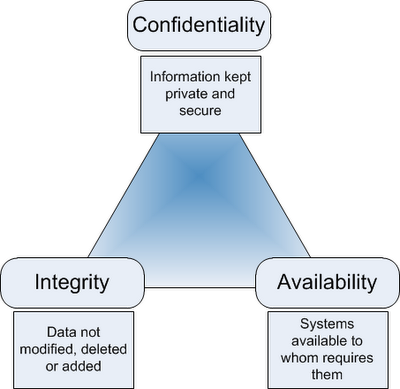
\includegraphics[width=.55\textwidth]{figuras/c-i-a.png}
  \caption[Elementos principales de seguridad de la información]{Elementos principales de seguridad de la información\\
  \footnotesize{Fuente: \textit{http://geraintw.blogspot.com.es/2012/09/cia-infosec.html}}}
  \label{fig:fundamentos-seguridad}
\end{figure}


\section*{Ejemplo de lista con números}

\begin{enumerate}

\item Confidencialidad:\\
El principio de confidencialidad consiste en asegurar que la información es accesible sólo para aquellos destinatarios que estén autorizados, con independencia de dónde se almacene la información.
La confidencialidad de los datos se implementa mediante mecanismos de control de acceso, tanto físicos (hardware) como  de programación (software).

\item Integridad:\\
La integridad de los datos se refiere a garantizar el estado de la información, protegiéndola de cambios accidentales o malintencionados. Mantener la integridad es esencial para la privacidad, la seguridad y la fiabilidad de los datos almacenados en un sistema.
Las medidas que se utilizan para mitigar posibles fallos en los datos incluyen: copias de seguridad regulares, almacenamiento seguro de esas copias fuera del lugar de trabajo y herramientas de control de integridad.

\item Disponibilidad:\\
La disponibilidad de los datos tiene como objetivo que los usuarios autorizados tengan acceso a la información en el momento que la necesiten. Esto implica garantizar el correcto funcionamiento de los equipos utilizados para almacenar y procesar los datos, de los controles de seguridad para protegerlos, y de los canales de comunicación utilizados para acceder a ellos.

\end{enumerate}


\section*{Una tabla con varias cabeceras}
\label{Ciberseguridad robótica}

La tabla~\ref{tabla1} extiende a los robots sociales y asistenciales la clasificación de criticidad para sistemas industriales, propuesta en \cite{CSSP}.

\begin{table*}[ht]
	\centering
	\caption{Perfiles de seguridad asociados a la robótica}
	\label{tabla1}
	\begin{tabular}{|l|ccc|}
		\cline{2-4}
		\multicolumn{1}{c}{} & \multicolumn{3}{|c|}{Criticidad} \\
		\cline{1-4}
		\multicolumn{1}{|c|}{Perfil} &  Confidencialidad & Integridad & Disponibilidad \\ \hline
		Estación de trabajo (PC) & Alta & Alta 	&  Baja \\
		Equipo para control industrial & Baja & Media & Muy alta \\
		Robots asistenciales & Muy alta & Muy alta & Muy alta \\
		Robots sociales & Muy alta & Media & Baja \\ \hline
	\end{tabular}
\end{table*}


\section*{Descripción de ROS: Robot Operating System}
\label{ROS}

Vistazo general sobre ROS:\\
- Historia y versión actual.\\
- Aplicación: investigación y también robots comerciales.\\
- Arquitectura: componentes básicos y funcionamiento.


\section*{Ejemplo de código fuente}

\vspace{0.5cm}  % Añado espacio vertical extra para separar el código del título de la sección.

\begin{lstlisting}
#!/bin/bash

# VARIABLES GLOBALES:

BASHRC_FILE="$HOME/.bashrc"
HOST_VAR_NAME="ROS_HOSTNAME"
MASTER_VAR_NAME="ROS_MASTER_URI"
ROS_PORT="11311"
HOST_IP=""    # Se asigna por parametro.
MASTER_IP=""  # Se asigna por parametro.
FILENAME="$(basename $0)"

# FUNCIONES:

description() {
if [ $1 -ne 0 ]; then
echo -e "\n  ========"
fi
echo -e "\n  This script adds or modifies $HOST_VAR_NAME and $MASTER_VAR_NAME variables"
echo -e "    in the '~/.bashrc' file of current user.\n"
}
\end{lstlisting}



%*********************************************

\chapter{Estudio del problema}
\label{Estudio del problema}

Se presenta el contexto de realización del trabajo realizando una revisión de las tecnologías, plataformas, herramientas o trabajos previos realizados en el mismo. Extensión aproximada de veinte páginas.

\section{El contexto del problema}

Breve descripción del contexto de realización del trabajo. Sirve para situar al lector.


\section{El estado del arte}

Para conocer el punto en el que se encuentran las investigaciones relacionadas con este trabajo que han sido realizadas anteriormente se realizará el estado del arte. La metodología de investigación se divide en las siguientes tres fases: planificación de búsqueda, proceso de búsqueda y selección de muestras, y extracción de datos y preparación de informes. Para realizar el estudio seguimos las recomendaciones de Kitchenham \cite{nueve}, así como la guía PRISMA \cite{diez}. 

\subsection{Definición del proyecto}

Tras comprobar que no se ha realizado un estudio centrado exactamente en el campo de interés de nuestro trabajo que responda a las preguntas planteadas en él, se ha procedido a la búsqueda de artículos de los que conforman el universo de estudio con el que se trabajará. Se han considerado varias fuentes de información tales como IEEE Digital Library y Scopus.

Una vez decididas las bases de datos en las que se van a realozar las búsquedas, es necesario construir cadenas de búsqueda adecuadas que permitan obtener resultados satisfactorios. Para la realización de la búsqueda se han construido XXX cadenas que se aplican a cada una de las bases de datos indicadas anteriormente. Se utilizarán artículos de acceso libre.

La primera de ellas juntando a todas las tecnologías para conocer si hay alguna información combinada de ambas

SS1('charging station' AND 'vehicle' AND ('security' OR 'cybersecurity') AND ('RFID' OR 'NFC'))

Mediante esta cadena de búsqueda se intentó recopilar un conjunto de artículos en los que se encuentren todos los términos del trabajo. Uno de los filtros que se aplican durante la búsqueda es el relacionado con la fecha de publicación del artículo. Al ser campos tecnológicos, con cambios muy veloces, como es la ciberseguridad, nos centraremos únicamente en artículos recientes. En este caso, la búsqueda se centra en artículos publicados entre el año 2019 a hoy.

Por otro lado se han realizado otras dos búsquedas separando las cadenas anteriores para conocer el estado de ambas tecnologías por separado dado que no hay una gran cantidad de artículos en la búsqueda anterior.

SS2(('security' OR 'cybersecurity') AND ('RFID' OR 'NFC'))
SS3('charging station' AND 'vehicle')

En este caso el tiempo de búsqueda es menor, ya que hay un mayor número de artículos y, como se ha mencionado anteriormente, las tecnologías NFC y los cargadores de coche eléctrico tienen una evolución muy rápida y constante.



\section{La definición del problema}

Los equipos de suministro de vehículos eléctricos (EVSE), también conocidos como estaciones de recarga, sirven para cargar los vehículos eléctricos. Los EVSE contienen sistemas de computación conectados a Internet. Estos sistemas cumplen importantes funciones de control, tales como la autorización, la recarga de vehículos eléctricos y la conexión a la red eléctrica local. Las estaciones de carga autorizan a usuarios y vehículos mediante tarjetas RFID o NFC, Bluetooth o Wi-Fi.

Por todo ello, hay muchos componentes de detección, comunicación y computación en los EVSE que son potencialmente vulnerables a los ataques de ciberseguridad. Como en todos los ataques, los piratas informáticos tratan de explotar estas vulnerabilidades para comprometer la disponibilidad, la integridad y la confidencialidad de la red. En este caso, se habla de una red de estaciones de carga o incluso la red eléctrica. Dado el tremendo crecimiento del mercado de vehículos eléctricos en los próximos años, es importante diseñar estaciones de carga confiables. El diseño de estaciones de carga confiables necesita una comprensión más profunda de las interacciones ciberfísicas dentro de la estación de carga, así como de las relaciones entre los componentes cibernéticos y físicos. 

Se presenta un enfoque de sistema para comprender los posibles ataques a este tipo de sistemas. Además se tratará el estado de los sistemas de carga inteligente y de los sistemas de comunicaciones NFC. Se propone una estructura de sistema basica para dirimir las autorizaciones para poder recargar basada en un servidor web y una base de datos. Finalmente se propondrá un sistema conceptual para evitar los ataques de acceso no autorizado a nivel físico al punto de recarga (robo de datos NFC o denegación de servicio (DoS) para mejorar la seguridad de estos sistemas.

\chapter{Estaciones de recarga del coche eléctrico (EVSE)}
\label{Estaciones de recarga del coche eléctrico (EVSE)}

En la próxima década se espera un gran crecimiento de los vehículos eléctricos enchufables (PEV) en el mundo. El calcula que en la próxima década habrá en circulación unos 120 millones de coches eléctricos. En lo que corresponde a España, actualmente se calcula que, en el mejor de los casos, no disponemos de más de 674 mil automóviles tanto eléctricos como híbridos. El equipo de carga, también conocido como Equipo de Suministro de Vehículos Eléctricos (EVSE) o estaciones de carga, proporciona carga segura a los vehículos eléctricos, de manera similar a las estaciones de servicio. 

Actualmente, una de las limitaciones más graves para la difusión de lPEV es la falta de una infraestructura de carga de PEV generalizada, a pesar de la gran difusión de la infraestructura eléctrica. Aunque se espera que el problema del coste de los PEV disminuya con su creciente difusión (lo que va produciendo una mayor investigación y avance en este tipo de tecnologías), la todavía limitada autonomía del automóvil y el aún largo tiempo de carga de la batería, mucho más prolongado en comparación con el que se tarda en rellenar el depósito de combustible de los vehículos de combustión interna \cite{diezuno}, son percibidos actualmente por los compradores como serias barreras a la compra \cite{diezdos}\cite{dieztres}.

Por ahora, el tiempo de recarga de la batería está limitado principalmente por la capacidad de la conexión a la red. Si bien la recarga mediante enchufes puede realizarse durante la noche en el hogar, es posible realizar una solución de recarga más rápida que requiere una alta potencia para la red eléctrica en estaciones de recarga, en estacionamientos públicos o comerciales, en centros comerciales y en la calle o los lugares de trabajo.

Con una difusión masiva del PEV, las cargas de las baterías tendrán un gran impacto en el funcionamiento de las redes inteligentes, por lo que se debería tener en cuenta la alta potencia necesaria para una carga rápida (por ejemplo, se requieren 150 kW para cargar un Tesla modelo S del 20\% al 80\% en 30 minutos). Los problemas de sobrecarga de la red eléctrica pueden surgir cuando varios vehículos en el mismo vecindario se recargan al mismo tiempo, o durante los picos de carga normales.

Los sistemas de carga de coche eléctrico no dejan de ser un tipo de sistema ciberfísico. Estos sistemas ciberfísicos (CPS, por sus siglas en inglés) son sistemas construidos mediante una integración segura y sin inconvenientes físicos y de computación (es decir, detección, computación y redes). Las llamadas tecnologías de sistemas inteligentes, como el transporte inteligente, la red inteligente, los vehículos inteligentes... se basan en los fundamentos de esta integración de CPS. La carga inteligente proporciona un mecanismo de comunicación entre el EVSE y la red que admite el monitoreo y la gestión de energía para mejorar la eficiencia y la personalización de los horarios de carga. A través de una mejor conectividad y control estos protocolos de carga inteligente han sido diseñados para reducir costes, equilibrar las cargas máximas y facilitar una mejor integración con diferentes niveles de operadores de red y fuentes de energía renovable. Los EVSE existentes tienen varios componentes tanto de comunicación como informáticos los cuales se utilizan para gestionar y controlar su funcionamiento. Por otro lado, las tecnologías emergentes de redes inteligentes también tienen como objetivo el facilitar un intercambio de energía bidireccional entre los vehículos eléctricos enchufables y la red a través de EVSE, en particular los cargadores rápidos. Además durante el proceso de autenticación para el inicio de la recarga inteligente se envían tanto la información personal como la financiera. Por todo ello, que la operación de EVSE sea segura es muy importante tanto para los vehículos como para las personas y la infraestructura de la red eléctrica.

Hay varias posibles motivaciones para lanzar un ataque a una estación de carga que van desde el robo de electricidad hasta algunos ataques más sofisticados buscan producir la interrupción de una red de estaciones de carga mediante el uso de un EVSE como punto de entrada a la misma. Los ataques podrían ser aún más graves si el malware consigue propagarse potencialmente a través de una red de estaciones de carga que pudieran afectar la red eléctrica.

La Sociedad de Ingenieros Automotrices (SAE) ha desarrollado un conjunto de estándares y protocolos para ser implementados por los fabricantes de estaciones de carga. La cantidad de componentes interconectados en EVSE y la conectividad de este con otros subsistemas (vehículos, smartphones, la red eléctrica...), y los mecanismos de seguridad mal implementados hacen que EVSE sea muy vulnerable a los ataques cibernéticos. El Departamento de Energía/Departamento de Transporte de los Estados Unidos (DOE/ DOT) realizó un informe el cual destaca brechas de seguridad cibernética en la infraestructura EVSE actual que incluye ataques de intermediarios o terceras personas, fraude de pagos, privacidad, daños a la batería del vehículo, deegación de servicio (DoS) y el malware se propaga del vehículo eléctrico o PEV al EVSE. El informe antes mencionado y algunos otros estudios \cite{once}\cite{doce}\cite{trece} demostraron algunas brechas y deficiencias en la infraestructura de carga existente por la falta de guías a seguir y pruebas de seguridad cibernética realizadas antes de su implementación. Además también indican algunos estudios cómo la carga descontrolada de EVSE puede crear un desequilibrio o un efecto negativo en la red eléctrica.


\section{Seguridad de los dispositivos EVSE desde un punto de vista ciberfísico}
\label{Seguridad de los dispositivos EVSE desde un punto de vista ciberfísico}

Actualmente, la mayoría de las estaciones de carga ya implementan algún tipo de seguridad de la información. Pero, en cualquier caso, estos métodos basados en tecnología de la información están limitados con respecto a la comprensión de cómo puede verse afectada la seguridad general de CPS. Relacionando los objetivos de ciberseguridad generales con los de este sistema encontramos lo siguiente:


\begin{enumerate}

\item \textit{Disponibilidad}: Está determinada por el tiempo activo frente al tiempo de inactividad de los servicios de carga. Es importante que se proporcione un sistema defensivo para monitorizar, detectar y prevenir ataques DoS, entre otros tipos de ataques a las estaciones de carga, para mantener una alta disponibilidad.
\item \textit{Integridad}: Es la protección contra cambios no autorizados, ya sea en los datos como en la información de control. La protección debe proporcionarse contra la manipulación de la información almacenada o intercambiada entre varias entidades, ya sea la estación de carga, el servidor centralizado o el dispositivo del cliente. 
\item \textit{Confidencialidad}: Garantiza el mantenimiento del secreto en la transmisión de datos entre las partes, ya sean datos del usuario o información bancaria.

\end{enumerate}

Los principales tipos de EVSE son el Nivel 1 (120V de corriente alterna, en adelante CA,  monofásico de ``carga lenta”), el Nivel 2 (240V de CA de fase dividida) y el Nivel 3 (hasta 500V de corriente continua, en adelante CC).El hardware de los EVSE de nivel 2 diseñados para su uso en estaciones de carga disponibles públicamente es bastante más complejo que los cargadores de nivel 1 y los EVSE de nivel 2 diseñados para uso doméstico privado. La disponibilidad de un hardware informático más sofisticado también permite que el EVSE de nivel 2 tenga un mayor número de protecciones de seguridad para la carga que la mayoría de los EVSE de nivel 1. Más allá del equipo necesario para iniciar la recarga de CA, el EVSE de nivel 2 en las estaciones de carga requiere placas de circuito impreso patentadas para controlar una variedad de componentes y subsistemas. Muchos EVSE de nivel 2 tienen módulos de comunicación que se utilizan para conectarse con una red de comunicaciones de forma inalámbrica, lo que permite a los fabricantes implementar una serie de funciones, como validación y verificación de usuarios, establecimiento de tarifas por parte del administrador de la estación de recarga y el reporte de eventos tales como información de diagnóstico, inicialización y finalización de recargas...

Los EVSE en las estaciones de carga de nivel 2 suelen disponer de indicadores LED y LCD que se utilizan para proporcionar a los usuarios información sobre el estado de la estación y/o la en qué estado se encuentra su proceso de carga, algo similar a las bombas de gasolina modernas. También es común que EVSE venga equipado con escáneres de identificación por radiofrecuencia (RFID) que pueden leer tarjetas de crédito o tarjetas de miembros de la red EVSE para poder procesar pagos. EVSE puede implementar varias placas con algunos propósitos especiales, ya sea una placa de comunicación, una placa de LED o una placa de E/S de usuario. 

El tener un hardware más sofisticado permite que el EVSE de nivel 2 pueda incluir más protecciones de seguridad para el proceso de recarga que la mayoría de los EVSE de nivel 1. Al igual que el EVSE de nivel 1, el EVSE de nivel 2 interactúa con los PEV a través de un conector de cinco conductores. Tres de los cables están conectados para suministrar energía desde la red eléctrica y solo están separados de una conexión directa de red al PEV a través de relés internos del EVSE. Se utiliza una combinación de tres tomas de voltaje conectadas directamente además de tres sensores de transformadores de corriente no invasivos que proporcionan al hardware de la computadora principal del EVSE información sobre la energía entregada a un vehículo conectado al punto de recarga, lo que permite las mediciones necesarias utilizadas para calcular el coste de la sesión de recarga. Los otros dos cables son la línea piloto y la línea de proximidad. La línea de proximidad se conecta solo a una red de resistencia simple dentro del enchufe EVSE que es la que el PEV utiliza para determinar si la conexión está bien realizada. Normalmente no se comunica con el hardware de la computadora EVSE de ninguna manera, aunque algunos modelos incluyen componentes electrónicos en el circuito que evitan que se notifique en el extremo PEV que la conexión se ha realizado correctamente cuando el EVSE no está listo para recargar. El cable más importante es la línea piloto, que es el que utilizan el EVSE y el PEV para comunicarse entre sí. Cuando una estación está inactiva, se aplica una señal de voltaje de 12V CC a la línea piloto, pero cuando un PEV consigue conectarse mediante una conexión física, el EVSE detecta esta acción a través de un detector de voltaje y cambia a una fuente que genera una onda cuadrada de 1kHz de amplitud de 12V en la línea piloto. Después, un circuito eléctrico en el PEV que consta de interruptores y resistencias responde a EVSE cuando se detecta esta onda cuadrada y el EVSE puede comenzar un proceso de recarga. Si se produce un problema eléctrico en el lado de la red del EVSE o si es el propio usuario el que desconecta repentinamente su vehículo del EVSE en medio de una sesión de recarga, el hardware de la computadora EVSE abrirá los relés en una fracción de segundo, eliminando la energía del adaptador para evitar cualquier tipo de daño al usuario.

El hardware de la computadora y el sensor de Level 3 EVSE es como el de Level 2 EVSE. Dos de los tipos principales de estaciones de carga rápida de CC son las que utilizan la expansión del estándar de carga combinada (CCS) y las que siguen el protocolo japonés CHAdeMO, junto con con los supercargadores patentados de Tesla Motor, que solo funcionan con sus propios vehículos, siendo el tercero más influyente. Las principales diferencias entre los EVSE de nivel 2 y 3 se reducen a la ubicación del circuito del cargador, el método de comunicación por cable entre el PEV y el EVSE, y el diseño del adaptador físico. Aunque se utiliza habitualmente de forma errónea el término ``cargador" para referirse a EVSE en publicaciones, todos los EVSE de nivel 3 que están en el mercado ya contienen rectificadores de CA-CC y otros circuitos de carga dentro del propio EVSE, mientras que la recarga de nivel 2 requiere dichos circuitos dentro del PEV. Los conectores físicos para CCS EVSE son esencialmente conectores modificados que incluyen dos pines grandes que se usan para la entrega de energía de CC. CCS EVSE puede utilizar la línea piloto igual que el EVSE de nivel 2, aunque este conductor se puede utilizar también para la comunicación por línea eléctrica (PLC) con la red inteligente. Los conectores CHAdeMO EVSE cuentan con un conjunto similar de dos pines grandes al adaptador CCS, pero también tienen una mayor cantidad de pines en total. Tres de estos son pines de control de sesión de carga que funcionan de igual forma que la línea piloto, pero dos de los pines se usan para facilitar la comunicación de la red de área del controlador con los vehículos, lo que habilita una comunicación por cable más compleja.

\section{Tipos de ataques centrados en dispositivos EVSE}
\label{Tipos de ataques centrados en dispositivos EVSE}

Una superficie de ataque es un punto de entrada a través del cual se pueden lanzar multitud de ataques. Hay dos categorías diferentes de puntos de entrada que podrían usarse para comprometer la seguridad de un EVSE: los físicos (utilizando el puerto de carga, manipulando el hardware de los dispositivos...) y los basados en la red.


\subsection{Ataques basados en la red}

Habitualmente los cargadores de nivel 2 y nivel 3 son equipados con algún módulo de comunicación con una interfaz inalámbrica (Bluetooth, Wi-Fi...) o por cable. Este módulo de comunicación permite a los usuario autorizados iniciar una sesión de recarga y a la propia estación de recarga comunicar su estado propio o el estado de la sesión de recarga al operador de la misma estación. Esta comunicación se produce a través de módulos en el vehículo, un teléfono inteligente o una tarjeta RFID. Las vulnerabilidades de las comunicaciones de corto y largo alcance están bien documentadas en la literatura [11-14]. Poner en peligro la seguridad de cualquiera de estos puntos finales de la red (es decir, BEMS, el servidor del controlador y la interfaz de operación de la estación) debido a una mala autenticación o falta de cifrado tiene el potencial de afectar a todas las estaciones de carga conectadas al nodo final. Esto tiene el potencial de comprometer la confidencialidad e integridad tanto de los datos como de los comandos de control, lo que afecta la disponibilidad de la estación de carga, el controlador de la estación de carga (o interfaz de gestión), el servidor BEMS y/o la red eléctrica. 
Una lista de posibles ataques basados en la red es la siguiente:



\begin{enumerate}

\item \textit{Suplantación de identidad}: La mayoría de las comunicaciones basadas en protocolos de comunicación inalámbrica (RFID, Bluetooth, Wi-Fi...) pueden sufrir este tipo de ataques. Una forma común de este ataque es comprometer el identificador único del dispositivo (por ejemplo, el tag RFID) y hacerse pasar por ese usuario (por tanto, un usuario legítimo). Esto suele ocurrir antes de que se establezca el cifrado y se generen las claves. Este tupo de ataques tienen la capacidad de comprometer la identidad del usuario (por tanto, atacar a su privacidad) y de modificar los datos transmitidos (atacar a la integridad de ellos). Para realizar un ataque por ejemplo se utilizaría la identidad del usuario para, por ejemplo, realizar la recarga en el nombre de otra persona o incluso para poder lanzar ataques DoS, los cuales se verán más adelante.

\item \textit{Man-in-the-Middle (Hombre en el medio, MITM)}:  El atacante trata de bloquear el receptor mientras puede acceder al tráfico transmitido, lo que permite que el atacante actúe como un punto intermedio entre el emisor y el receptor sin que ninguna de las partes lo sepa. La mayoría de las comunicaciones basadas en radio son propensas a estos ataques MITM. Estos pueden ocurrir entre los nodos (por ejemplo EVSE y PEV). El atacante podría corromper los datos o tomar el control completo del nodo y alterar el estado de uno de ellos para por ejemplo transmitir información incorrecta (por ejemplo notificar en la estación de recarga un error que no existe). Si las comunicaciones o el código fuente no se ofuscan o encriptan los ataques MITM son más fáciles de ejecutar.

\item \textit{Denegation of Service (Negación de Servicio, DoS)}: Si se comprometen las credenciales del usuario, el propio usuario y la estación se podrían utilizar para lanzar ataques DOS muy sofisticados. Por ejemplo, las credenciales de usuario se pueden usar para lanzar este tipo de ataques contra nodos. Los posibles ataques a considerar son la inundación UDP o TCP/IP, DoS de baja velocidad, inundación de ping o inundación ICMP. Estos ataques son capaces pueden deshabilitar una estación de carga u otros nodos situados en la misma red de la estación de carga.

\item \textit{Ataque de inyección SQL}: Explota una base de datos con una implementación no del todo correcta para insertar, actualizar o eliminar datos de la propia base de datos. Esto haría que un atacante pueda ejecutar comandos que afecten a, entre otras cosas, la capacidad de recarga de los usuarios, imposibilitar el acceso a algún usuario, cambiar la disponibilidad de una estación, robar datos económicos... lo que puede causar problemas de seguridad o económicos.

\item \textit{Ataque de malware}: Explota una mala implementación de seguridad de varios de los módulos de software en la estación de carga y o en la nube para lanzar ataques más sofisticados que instalen algún tipo de malware. Por ejemplo, un malware con potencial de lanzar un ataque más coordinado podría provocar el cierre de una red de estaciones de carga o hasta afectar a toda la red eléctrica porque se podrían activar varias estaciones de carga simultáneamente.

\end{enumerate}



\subsection{Ataques físicos}

En teoría, un atacante que disponga de acceso físico a un EVSE podría recoger información de la placa de la estación de carga para espiar las comunicaciones entre componentes. Esto se podría hacer manipulando físicamente la estación de carga si la resistencia a ella es débil. Dado que cada tipo de EVSE tiene una arquitectura diferente, el atacante debe estudiar diferentes componentes, comprender varios módulos de comunicación de la estación de carga y tener algún tipo de microcontrolador y varias herramientas de rastreo o sondeo para obtener información valiosa de su acceso físico a la estación de carga. La complejidad de la arquitectura varía mucho entre cada tipo de EVSE. Todas las estaciones de carga de nivel 2 y nivel 3 tienen un microcontrolador para controlar las funciones requeridas por un EVSE, y muchas están equipadas con un sistema operativo en tiempo real que habitualmente ejecuta un núcleo Linux. Existen varias herramientas de hardware para extraer firmware a través de las interfaces \textit{Universal Asynchronous Receiver- Transmitter} (UART) o \textit{Joint Test Action Group} (JTAG). Los tipos específicos de ataques incluyen los siguientes:


\begin{enumerate}

\item \textit{Físicos y de canal lateral}: Implican obtener acceso a los componentes de nivel de chip para manipular e interferir con las partes internas del sistema. Junto con este tipo de ataque, los hay de canal lateral que implican la ingeniería inversa de un chip al observar información de tiempo, consumo de energía y fugas electromagnéticas. Con esta información, es posible recuperar datos confidenciales, como por ejemplo claves de cifrado utilizadas en las comunicaciones o datos que se transmiten a través de la electrónica de la estación de recarga. Estos ataques son muy difíciles de implementar y requieren equipos con un coste elevado.

\item \textit{Basados en interceptación}: Implica el espionaje de datos confidenciales, lo que compromete la privacidad y confidencialidad del usuario. Esto se logra mediante el uso de técnicas de sondeo para acceder y monitorear los datos en los puertos del hardware físico. Además se puede usar también para interceptar algún tipo de información enviada al EVSE, lo que podría alterarla antes de que se envíe al sistema.

\item \textit{Basados en modificación}: Compromete integridad del software mediante la explotación de las vulnerabilidades detectadas. Por ejemplo, el acto de usar un desbordamiento de búfer para sobrescribir la memoria de la pila, dirigiendo el control hacia algún programa de tipo malware, constituiría un ataque de modificación.

\end{enumerate}



\subsection{Ataques híbridos}

Mediante el uso de varias combinaciones de ataques basados en la red red y ataques físicos, es posible lanzar ataques aún más sofisticados. Por ejemplo, si un atacante tuviera acceso al servicio en la nube, se podría autorizar un EVSE para iniciar una sesión de recarga con un vehículo manejado por un usuario no autorizado. Para los EVSE que carecen de un protocolo de enlace PEV-EVSE correctamente implementado al contacto, la modificación física del enchufe del adaptador del EVSE permite activar una sesión de carga de Nivel 2 sin la presencia de l vehículo. La combinación de ambos ataques permite que el enchufe del adaptador de la estación de carga se active remotamente, lo que podría permitir que algunos dispositivos distintos a los PEV reciban energía a través del EVSE, pudiendo utilizarse esto para cualquier fin.

Los diferentes ataques que pueden realizarse a partir de la combinación de ataques físicos y cibernéticos a la red pueden ser increíblemente perjudiciales para el funcionamiento normal de un EVSE y la seguridad de los usuarios.


\section{Enfoques para mejorar la seguridad CPS}
\label{Enfoques para mejorar la seguridad CPS}

Se están implementando e instalando una gran cantidad de puntos de recarga, de momento con estándares limitados para aportar seguridad a este tipo de infraestructuras. Dado que la seguridad y la disponibilidad de las estaciones de carga afectan indirectamente tanto a la red eléctrica como al sector del transporte, es importante disponer de unas bases sólidas de ciberseguridad para poder implementarlas. Algunas de ellas se adoptaron de las mejores prácticas de seguridad del sistema integrado, pero la mayoría de ellas son exclusivas de las propias estaciones de carga.

\subsection{Seguro por diseño}

El diseño de una estación de carga segura va mucho más allá de asegurar los componentes individuales del sistema. Esto se debe a que las estaciones de carga interactúan con múltiples sistemas, entre ellos vehículos, smartphones, la infraestructura energética y la nube. Estolo que hace es aumentar los vectores de amenazas, los cuales los atacantes pueden explotar. El diseño de seguridad de la estación de carga debe identificar todos los posibles vectores de amenazas (tanto cibernéticos como físicos), así como las vulnerabilidades y el riesgo que las amenazas supondrían para las personas, los vehículos y la infraestructura. Este dise;o debe incluir componentes tanto de hardware como de software. Los diseñadores de EVSE deben tener en cuenta la variedad de posibles amenazas y considerar las estrategias necesarias para limitarlas. Varios modelos gráficos y formales como Petrinets, diagramas de flujo de datos, simulaciones de eventos discretos o los modelos CPS \cite{catorce}\cite{quince}\cite{dieciseis}\cite{diecisiete} se pueden utilizar para verificar y evaluar las propiedades de seguridad y protección del diseño. Es necesaria además la existencia de un aislamiento limpio en el hardware y el software para evitar el acceso no autorizado o el espionaje de la información protegida y las señales de control.


\subsection{Seguridad del software}

La estación de carga incluye software que se ejecuta en la placa que envía las señales de control a la propia estación de carga, la interfaz de administración de la propia estación de carga, las aplicaciones móviles y la interfaz de programación de aplicaciones proporcionada por las estaciones de carga. La mayoría de estas estaciones también ofrecen un servidor que se comunica con la estación a través de Internet. Los principios de seguridad por diseño se aplican a la arquitectura de software para la estación de carga para identificar las lagunas de seguridad que hacen que estos sistemas sean vulnerables \cite{catorce}. Dada la integración compleja y estrecha de hardware y software, algunos de los ataques de software también se pueden realizar a través del hardware. Hay muchas contramedidas disponibles para autenticar y validar el software en diferentes pasos, como por ejemplo evitar la manipulación del software y asegurar el arranque.

\subsection{Seguridad del hardware}

Los microprocesadores que se utilizan en las estaciones de carga suelen tener una potencia computacional baja la cual es incompatible con implementar un cifrado fuerte. El agregar coprocesadores seguros como aceleradores de hardware criptográfico \cite{quince} reducirá las opciones de manipulación del hardware. Los coprocesadores seguros brindan soporte criptográfico de alto rendimiento que almacena claves de manera mucho más segura a pesar de los posibles ataques físicos o lógicos.


\subsection{Supervisión y resistencia a la manipulación}

El software malicioso también puede aprovechar las lagunas del software y del sistema operativo para instalar malware que afecte al funcionamiento normal del sistema. Las medidas de resistencia a la manipulación para proteger contra ataques físicos y de canal lateral incluyen protección física para evitar la manipulación, encriptación de BUS, implementación de circuitos donde las características de potencia son independientes de los datos y blindaje de los chips en la placa. Además de la protección contra manipulaciones, también es importante monitorizar y registrar las actividades críticas para prevenir e investigar algunas vulnerabilidades relacionadas con la seguridad cibernética.



\section{Estándar de protocolo de punto de recarga abierto (Open Charge Point Protocol, OCPP)}
\label{Estándar de protocolo de punto de recarga abierto (Open Charge Point Protocol, OCPP)}

La estandarización de los protocolos de comunicación para la movilidad eléctrica es necesaria para garantizar que el rendimiento, la seguridad y la protección sean los mismos que los del vehículo convencional real. Las principales organizaciones que desarrollaron estándares para los PEV son la Comisión Electrotécnica Internacional (IEC), la Sociedad de Ingeniería Automotriz (SAE), y otros consorcios públicos y empresas privadas de vehículos eléctricos que desarrollan estándares abiertos.

Existen diferentes estándares en continuo desarrollo en lo que respecta a la comunicación entre los PEV y los EVSE. Los principales estándares son \cite{quinceuno}\cite{quincedos}:

\begin{enumerate}

\item \textit{SAE J2931, SAE J2836, SAE J2847, SAE J1772}
\item \textit{CEI 61850-7-420, CEI 62196, CEI 61851, CEI 15118}
\item \textit{OCPP, OICP, OCHP}

\end{enumerate}

Para la realización del trabajo se utilizará el protocolo OCPP. OCPP \cite{quincedos}\cite{quincetres} es un estándar abierto creado por Open Charge Alliance (OCA), que consiste en un consorcio de varias organizaciones públicas y privadas.

OCPP es el estándar respaldado de facto por la industria para la comunicación entre una estación de carga y un sistema de gestión de estaciones de carga (CSMS) y está diseñado para adaptarse a cualquier tipo de técnica de carga \cite{quincetres}.

El objetivo de OCA es favorecer el desarrollo de una infraestructura de red con la creación de un protocolo abierto, libre e independiente de las características de cada fabricante individual, y que permita la gestión de todas las situaciones de una operación de recarga. El OCPP tiene como objetivo realizar una serie de operaciones entre componentes que representan dispositivos físicos involucrados en la operación de recarga. Estas operaciones se realizan mediante el intercambio de uno o más mensajes denominados Protocol Data Unity (Unidad de Datos de Protocolo, PDU).

La versión 1.5 de OCPP, de junio de 2012, es capaz de:

\begin{enumerate}

\item Monitorizar y controlar el acceso a las estaciones de carga individuales.
\item Consultar y gestionar el estado de la recarga.
\item Enviar datos a usuarios y administradores.
\item Permitir el procedimiento de pago.
\item Permitir mecanismos de reserva y gestión eléctrica.

\end{enumerate}


\chapter{Gestión de proyecto software}
\label{Gestión de proyecto software}

Realizar una simulación de la gestión del proyecto software desarrollo. La gestión simulará un proyecto real, realizado con las condiciones habituales del entorno empresarial. El objetivo del capítulo es plasmar los conocimientos adquiridos a lo largo de la titulación y no la forma en la cual se ha gestionado el Trabajo Fin de Máster. Extensión máxima de veinte páginas.

\section{Alcance del proyecto}
\label{Alcance del proyecto}

\subsection{Definición del proyecto}

\subsection{Estimación de tareas y recursos}

\subsection{Presupuesto}

A continuación se detalla un presupuesto estimado para el coste total de este proyecto.

\subsubsection{Coste de personal}

\begin{table*}[ht]
	\centering
	\caption{Presupuesto de personal}
	\label{tabla2}
	\makebox[\textwidth]{  % Para centrar una tabla más ancha que la página definida.
		\begin{tabular}{|c|c|c|c|c|}
			\cline{1-5}
			Tarea &	Perfil & Horas & Euros/Hora  &  Total\\ \hline
			Desarrollo aplicación &	Programador Junior & 80 & 60 & 4800 \euro\\
			Integración en entorno robótico & Programador Senior & 20 & 100 & 2000 \euro\\
			Pruebas & Ingeniero de Pruebas & 20 & 80 & 1600 \euro\\
			Supervisión del Proyecto & Jefe de Proyecto & 10 & 120 & 1200 \euro\\ \hline\hline
			\multicolumn{4}{|c|}{Total} & \multicolumn{1}{c|}{10100 \euro}\\ \hline
		\end{tabular}
	}
\end{table*}


\subsubsection{Coste del hardware}

Para la realización de este proyecto se ha realizado la compra de:

\begin{enumerate}
	
	\item Ordenador con Intel i7:
	
	Placa base: MSI GE62 6QF-060ES Heroes Ed.
	
	Procesador: Intel i7-6700HQ
	
	RAM: 16 GB
	
	Disco duro: 1TB + 128GB SSD
	
	Tarjeta gráfica: Nvidia GTX970M
	
	Monitor: 15.6"
	
	\begin{itemize}
		\item Precio (sin IVA): 986,71 \euro\\
	\end{itemize}
	
	\item Ordenador con Intel Atom:
	
	Asus Transformer Book H100TAM DK028B
	
	RAM: 32GB
	
	Disco duro: 500GB
	
	\begin{itemize}
		\item Precio (sin IVA): 260,27 \euro
	\end{itemize}
	
\end{enumerate}


\subsubsection{Coste total}

\begin{table*}[ht]
	\centering
	\caption{Presupuesto total}
	\label{tabla3}
	\makebox[\textwidth]{  % Para centrar una tabla ancha.
		\begin{tabular}{|l|l|}
			\cline{1-2}
			Concepto &	Coste (Euros) \\ \hline
			Costes de personal & 10100  \\
			Costes de hardware  & 1246,98   \\ \hline
			Subtotal  &  11346,97 \\
			IVA (21\%) & 2882,86 \\ \hline \hline
			Total Proyecto & \textbf{13729,83 \euro} \\ \hline
	\end{tabular}}
\end{table*}

\section{Plan de trabajo}
\label{Plan de trabajo}


\subsection{Identificación de tareas}

\subsection{Estimación de tareas}

\subsection{Planificación de tareas}



\section{Gestión de recursos}

\subsection{Especificación de recursos}

\subsection{Asignación de recursos}




\section{Gestión de riesgos}

\subsection{Identificación de riesgos}

\subsection{Análisis de riesgos}



\chapter{Solución}
\label{Solución}

Explicación de la solución llevada a cabo. Si se trata de un desarrollo se incidirá en el proceso de desarrollo; en otro caso, se justificará y describirá la solución propuesta. El capítulo tendrá una extensión aproximada de cuarenta páginas y, en ningún caso, excederá las cincuenta.

\section{Descripción de la solución}

Breve descripción del tipo de solución adoptada: si es una aplicación y qué características tiene, si se trata de un tutorial, un modelo, etc.


\section{El proceso de desarrollo}

Explicar el modelo de proceso y la estructura de la sección.

\subsection{Análisis}

Fase de análisis


\subsubsection{Definición de requisitos}

Enumerar los requisitos del sistema dividiéndoles en funcionales y no funcionales.

\subsubsection{Especificación de requisitos}

Analizar y especificar los requisitos desde el punto de vista del comportamiento, estructura y funcionalidad del sistema.


\subsection{Diseño}

Fase de diseño

\subsubsection{Diseño de sistema}

Se expone la ARQUITECTURA del sistema y las TECNOLOGÍAS utilizadas en el desarrollo.

\subsubsection{Diseño detallado}

Se describe el diseño de las capas de PERSISTENCIA, MODELO e INTERFAZ del sistema.


\subsection{Implementación}

Hablar de las HERRAMIENTAS utilizadas durante el desarrollo, la ORGANIZACIÓN del proyecto y aquellas peculiaridades de la forma de implementación.

\subsection{Pruebas}

Centrarse en pruebas unitarias (no incluir todas las pruebas sino informes de las mismas) y de sistema (mostrar que cumple los casos de uso).


\section{El producto del desarrollo}

En el caso de desarrollar una herramienta es necesario mostrar, brevemente, el tipo de herramienta generada. Incluir algún pantallazo de la herramienta, su funcionalidad y la forma de ejecución de la misma.

\chapter{Evaluación}
\label{Evaluación}


Demostración de la validez de la solución elaborada. La solución se considera válida si resuelve los problemas expuestos en el planteamiento del problema y satisface los objetivos definidos en la introducción. Según el caso la forma de evaluación se basará en la ejecución de casos de prueba o en la realización de cuestionarios. Extensión entre quince y veinte páginas.

\section{Proceso de evaluación}

\subsection{Forma de evaluación}

Explicar la forma en la cual se ha evaluado la aplicación

\subsection{Casos de prueba}

Casos de pruebas realizados

\section{Análisis de resultados}



\mychapter{1}{Conclusión}

Expresión personal del conjunto de conclusiones que, a juicio del autor, se derivan de los resultados expuestos en el trabajo.Deberá tener una extensión entre cinco y diez páginas.

\subsection*{Aportaciones realizadas}



\subsection*{Trabajos futuros}



\subsection*{Problemas encontrados}



\section*{Opiniones personales}



%%%% BIBLIOGRAFÍA %%%%
\bibliographystyle{splncs.bst}  % Fichero con el formato de la bibliografía.

\renewcommand\bibname{Lista de referencias}

%\bibliography{Refs-proyecto}    % Fichero con las referencias.
Información bibliográfica citada en el texto del trabajo. Otras lecturas recomendadas o consultadas, de figurar, aparecerán en anexos.
Se debe seguir la norma ISO 690 (buscar en google ISO 690 ugr)

% También se puede optar por incluir las referencias desde aquí mismo:
\begin{thebibliography}{1}
	
\bibitem{uno} \textit P. V. Nikitin, K. V. S. Rao y S. Lazar, ``An overview of near field UHF RFID", IEEE RFID. Conferencia, 2007, p\'ags.167-174.
\bibitem{dos} \textit M. M. Singh, K. A. A. K. Adzman, y R. Hassan, ``Near Field Communication (NFC) Technology Security Vulnerabilities and Countermeasures", International Journal of Engineering \& Technology Vol.7, N\textdegree 4.31, p\'ags.298-305, 2018.
\bibitem{tres} \textit ISO/IEC 18092. ``Near Field Comunication: interface and protocolo", 2004.
\bibitem{cuatro} \textit ECMA International (2005). ``Near Field Communication - White Paper”, Ecma/TC32-TG19/2005/ 012, 2005.
\bibitem{cinco} \textit ``NFC Data Exchange Format (NDEF), NFC Forum Technical Specification”
\bibitem{seis} \textit ``NFC-Near Field Communication, Reader/Writer Operating Mode”
\bibitem{siete} \textit Fahrianto F., Lubis M. F. y Fiade A., ``Denial-of-service attack possibilities on NFC technology”, 2016 4th International Conference on Cyber and IT Service Management, IEEE, págs.1-5, 2016
\bibitem{ocho} \textit Eun H., Lee H. y Oh H., ``Conditional privacy preserving security protocol for NFC applications”, IEEE T. Cons. Electr., Vol.59, N\textdegree.1, págs.153-160, 2013
\bibitem{nueve} \textit Kitchenham, B.A., Budgen, D., Brereton, P. ``Evidence-Based Software Engineering and Systematic Reviews”, vol. 4. CRC Press (2016)
\bibitem{diez} \textit Moher, D., Liberati, A., Tetzlaff, J., Altman, D.G., ATP Group. ``Preferred reporting
items for systematic reviews and meta-analyses: The PRISMA statement”. Ann. Internal Med. 151(4) (264–269), 2009.
\bibitem{diezuno} \textit Saalfeld, C. ``E-Mobility–Vehicle2Grid Interface. Vector-Kongress”, 2010
\bibitem{diezdos} \textit Bedogni, L., Bononi, L., Di Felice, M.; D’Elia, A.; Cinotti, T.S., ``A Route Planner Service with Recharging
Reservation: Electric Itinerary with a Click”. IEEE Intell. Transp. Syst. Mag. (8, 75–84), 2016.
\bibitem{dieztres} \textit Bedogni, L., Bononi, L., D’Elia, A., Di Felice, M., Rondelli, S., Cinotti, T.S. ``A Mobile Application to Assist
Electric Vehicles’ Drivers with Charging Services” (78–83). En las actas de la Eighth International Conference on Next Generation Mobile Apps, Services and Technologies, Oxford, UK, 10 al 12 de septiembre de 2014.
\bibitem{once} \textit Rhode, K. ``Electric Vehicle Cyber Research SANS Automotive Cybersecurity Workshop”, 2017
\bibitem{doce} \textit Shezaf, O., ``Who can hack a plug? The Infosec Risks of Charging Electric Cars”, 2013.
\bibitem{trece} \textit Fearn, F. Kaspersky, V3 news, ``Warning over electric car charging”, Enero de 2018.
\bibitem{catorce} \textit Kocher, Paul, et al. ``Security as a new dimension in embedded system design.” Actas de la 41.ª Conferencia anual de Automatización del Diseño. ACM, 2004.
\bibitem{quince} \textit Khelladi, Lyes, et al. ``On security issues in embedded systems: challenges and solutions.” International Journal of Information and Computer Security 2.2, 2008.
\bibitem{quinceuno} \textit Buamod I., Abdelmoghith E.,  Mouftah H.T., ``A review of OSI-based charging standards and eMobility open protocols”. En actas de la 2015 International Conference on the Network of the Future, NOF 2015, Montreal, QC, Canada, del 30 de septiembre al 2 de octubre del 2015.
\bibitem{quincedos} \textit Schmutzler J., Andersen C.A., Wietfeld C., ``Evaluation of OCPP and IEC 61850 for smart charging electric
vehicles”. World Electr. Veh. J., 2013
\bibitem{quincetres} \textit Home - Open Charge Alliance. Web: https://www.openchargealliance.org/.
\bibitem{dieciseis} \textit Wan, Kaiyu, K. L. Man, y D. Hughes. ``Specification, Analyzing Challenges and Approaches for Cyber-Physical Systems (CPS).” Engineering Letters 18.3, 2010.
\bibitem{diecisiete} \textit Orojloo, Hamed, y Mohammad Abdollahi Azgomi. ``A method for modeling and evaluation of the security of cyber-physical systems.” Information Security and Cryptology (ISCISC), 11ª Conferencia Internacional ISC sobre IEEE, 2014.

\bibitem{CSSP}
{CSSP, D.}:
\newblock \textit{Recommended Practice: Improving Industrial Control Systems
  Cybersecurity with Defense-In-Depth Strategies}.
\newblock US-CERT Defense In Depth. (Octubre 2009)

\end{thebibliography}



%%%% ANEXOS %%%%
\renewcommand{\appendixname}{Anexo}
\appendix

\chapter{Control de versiones}
\label{Control de versiones}




\chapter{Seguimiento de proyecto fin de máster}
\label{Seguimiento de proyecto fin de máster}


Obligatorio. Seguimiento del trabajo real.

\section{Forma de seguimiento}

\section{Planificación inicial}

\section{Planificación final}
Si el trabajo ha consistido en la elaboración de una aplicación se incluirá el manual de usuario de la misma.


\chapter{Cuestionario de evaluación}
\label{Cuestionario de evaluación}

Cuestionarios utilizados durante la fase de evaluación.



\end{document}
